\section{Introduction}


\begin{figure*}[t]
        \centering
        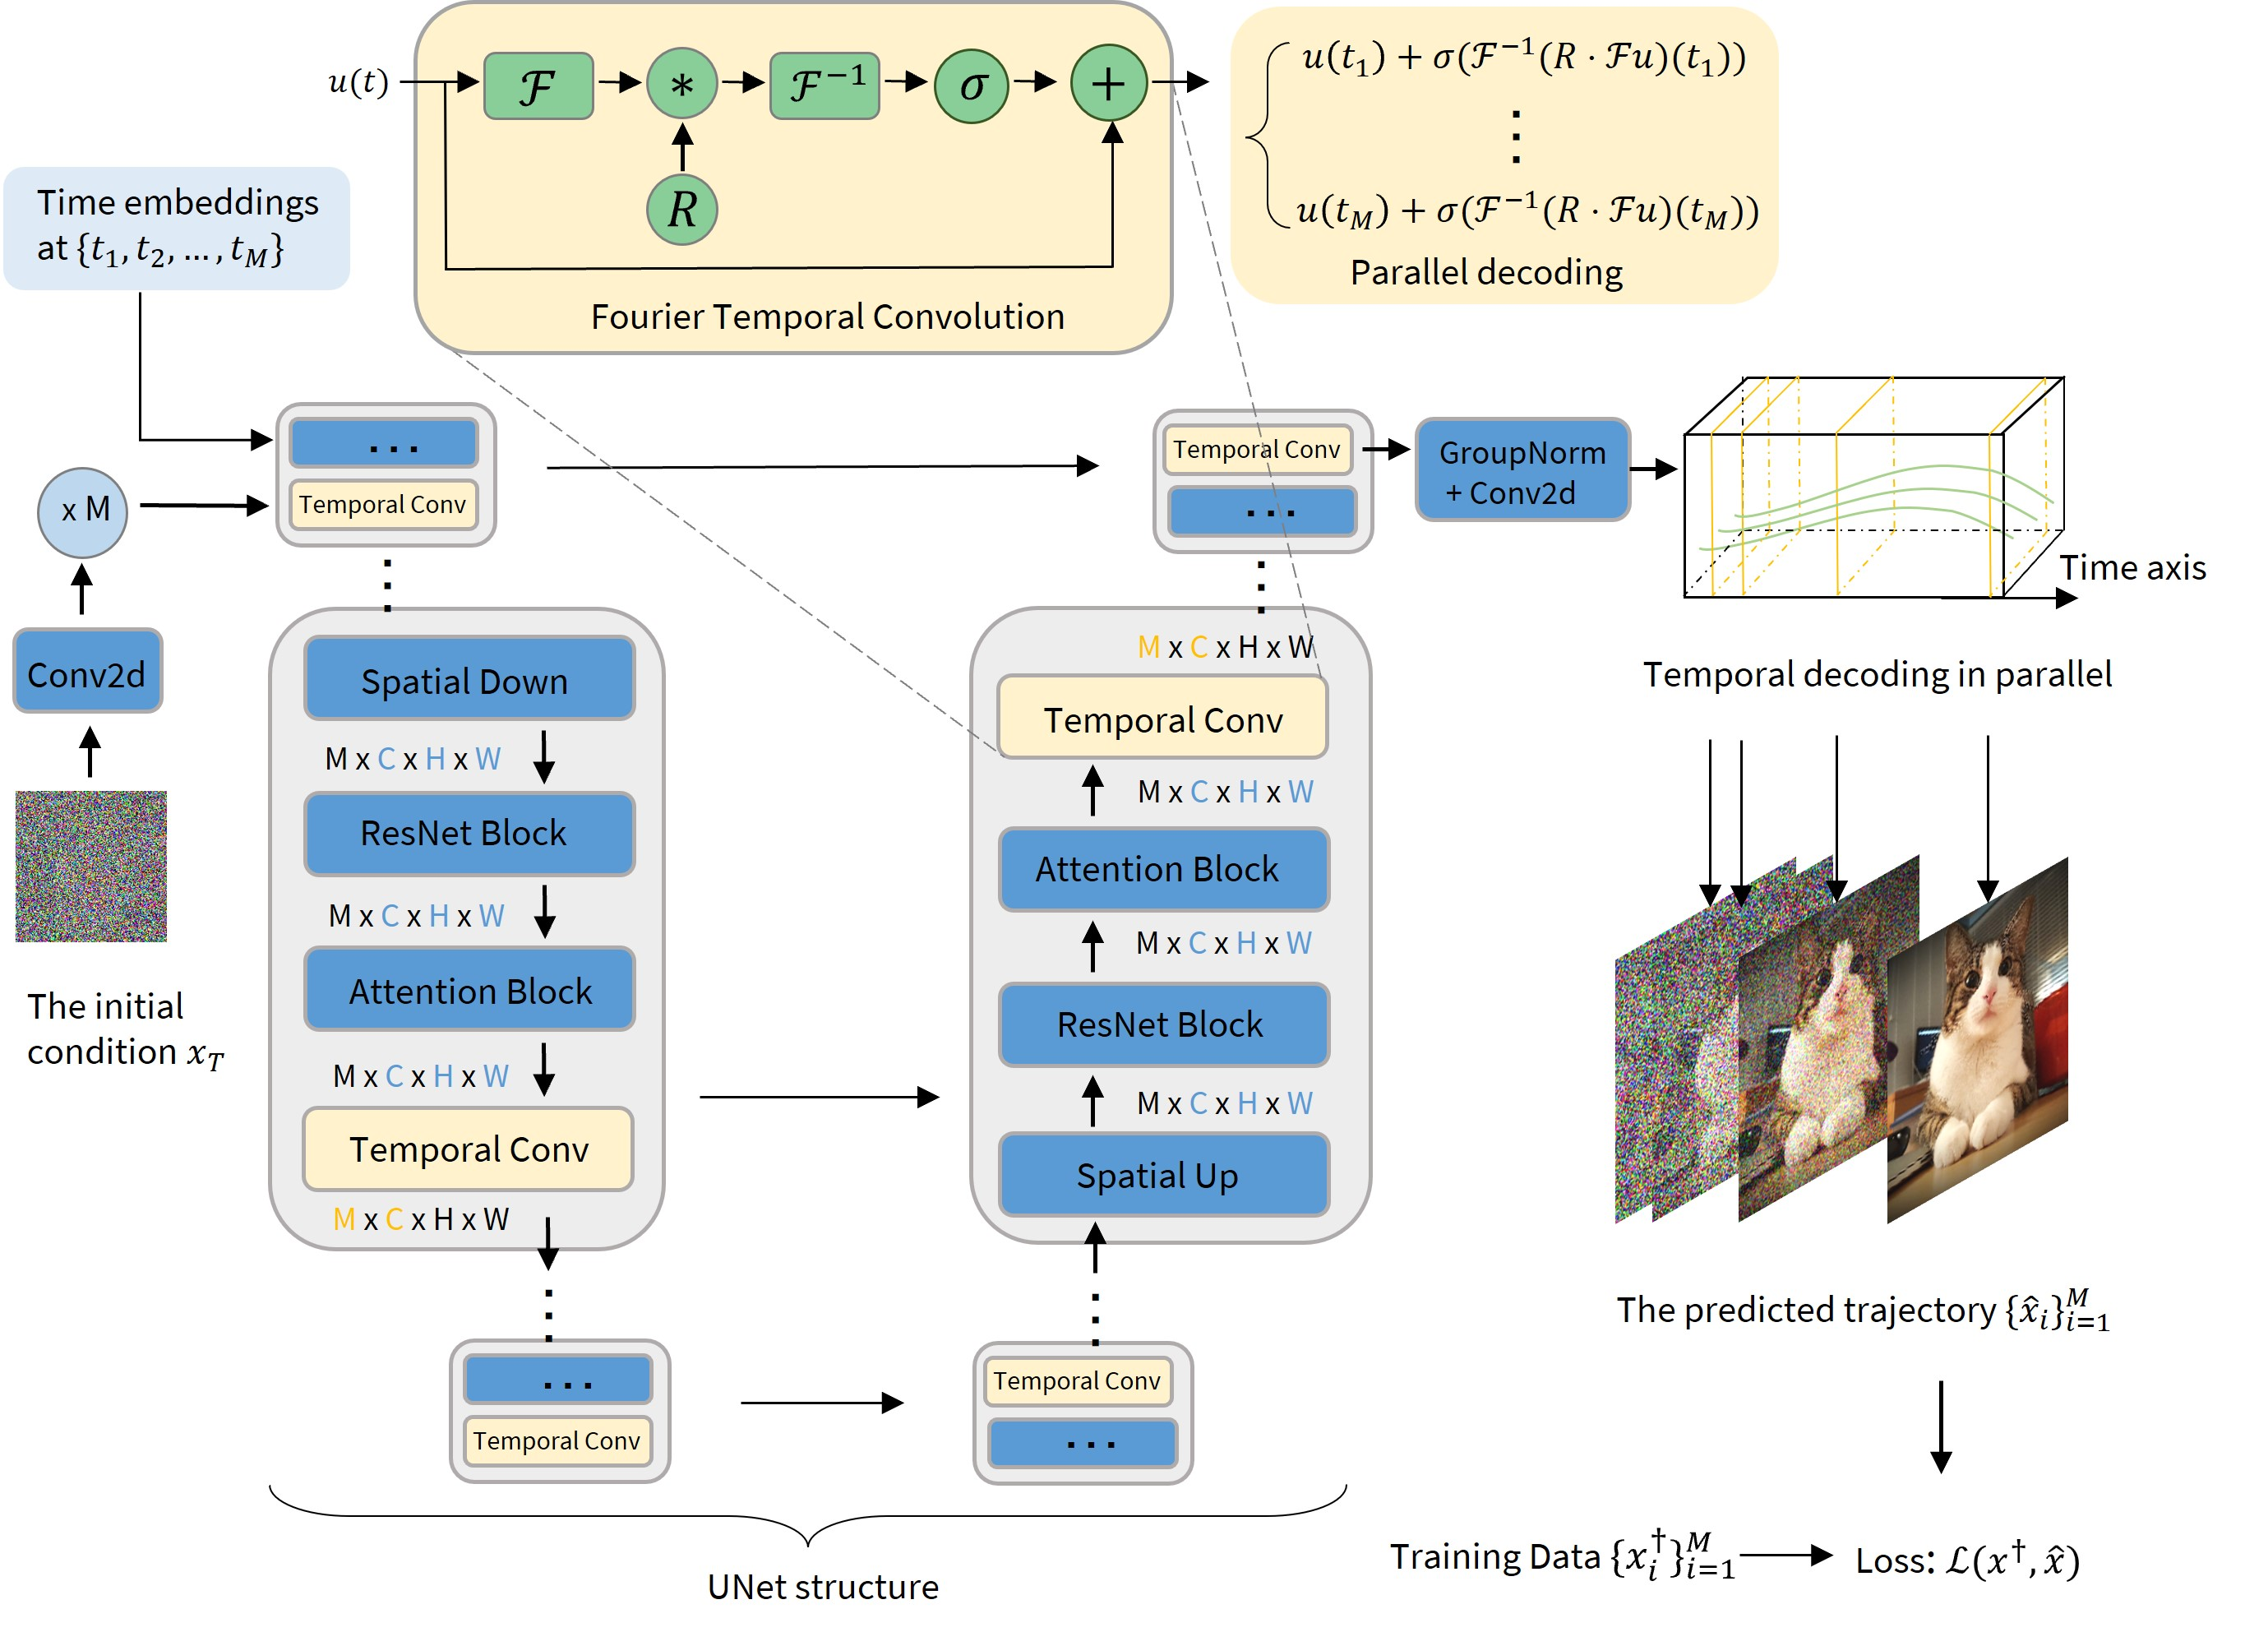
\includegraphics[width=0.92\textwidth]{figs/arch_v3-3.jpg}
        \caption{Illustration of the architecture and training pipeline of DSNO. The architecture of DSNO is built on top of any existing diffusion model architecture, where blue blocks are from the existing diffusion U-Net backbone and yellow blocks are the proposed temporal convolution layers.
        % introduced at each level of the UNet backbone. 
        % As indicated by the highlighted dimensions of the feature map, 
        Suppose the temporal domain is discretized into $M$ points $\{t_1,\dots,t_M\}$,
        % which is not necessarily a uniform grid,
        for each feature map, the temporal convolution layers operate on the temporal and channel dimensions (M$\times$C) and the other blocks operate on the pixel and channel dimensions (C$\times$H$\times$W). The symbols $\gF$ and $\gF^{-1}$ refer to the Fourier transform and inverse Fourier transform, respectively. 
        $R$ is a complex-valued parameter that represents a kernel function in Fourier space. For ease of notation, $x_i$ represents the solution at time $t_i$, that is $x(t_i)$. 
        Inside each temporal convolution layer, we apply the idea of parallel decoding: Given input function $u(t)$, the Fourier coefficients $R\cdot \gF u$ is the same for all $t_i, i=1,\dots, M$. Therefore, the temporal convolution layer can output the representations at different time locations in the trajectory in a single forward pass by evaluating the output function at queried points in parallel.}
        \label{fig:dfno_arch}
\end{figure*}




Diffusion models~\citep{sohl2015deep,ho2020denoising}, also known as score-based generative models~\citep{song2020score}, have emerged as a powerful generative modeling framework in various areas. They have achieved state-of-the-art (SOTA) performance in many applications including image generation \cite{dhariwal2021diffusion}, molecule generation \cite{xu2022geodiff}, audio synthesis \cite{kong2021diffwave} and model robustness~\cite{nie2022DiffPure}. However, sampling from diffusion models requires hundreds of neural network evaluations, making them slower by orders of magnitude compared to other generative models such as generative adversarial networks (GANs) \cite{goodfellow2020generative}. Accelerating sampling in diffusion models remains a challenging but important problem, especially when applying them to time-sensitive downstream applications such as AI for art and design \cite{ramesh2022hierarchical} or generative models for decision making \cite{ajay2022conditional}. 

Existing methods for fast sampling of diffusion models can be summarized into two main categories: 1) \emph{training-free sampling methods}~\citep{song2020denoising,lu2022dpm} and 2) \emph{training-based sampling methods}~\citep{luhman2021knowledge,salimans2021progressive,xiao2021tackling}. Specifically, the training-free methods focus on reducing the number of discretization steps from a numerical perspective while solving the stochastic differential equations (SDE) or probability flow ordinary differential equations (ODE). However, even the best well-designed numerical solvers \cite{lu2022dpm, karras2022elucidating} still need 10$\sim$30 model evaluations such that the approximation error is small enough for an acceptable sampling quality.
% generating reasonable-quality samples, which is still a big gap from real-time sampling. 
On the other hand, training-based methods train a  surrogate network to replace some parts of the numerical solver or even the whole solver. Particularly, progressive distillation \cite{salimans2021progressive} has made a big step towards real-time sampling (e.g., decent results with 4 steps) but it still has a sequential nature like conventional numerical solvers. %and comes at the price of a high training cost. 

 % Most prior works including training-based methods follow the structure of numerical solvers and solve the equation step by step. 
The goal of this work is to develop a fast and parallel sampling method for diffusion models \emph{with only one model evaluation}. By parallel, we mean that our method can decode images at different time locations in the trajectory in parallel and hence, generate the final solution using only one model evaluation. The major challenge here arises from the difficulty of solving a complicated and large-scale differential equation, which typically requires many discrete time steps to emulate accurately from a numerical approximation perspective. 

% On the contrary, the recent advancements in operator learning for solving differential equations open new doors to solving differential equations. 
In this paper, we employ the recent advances in neural operators for solving differential equations to overcome this challenge. 
Neural operators \citep{li2020neural,kovachki2021neural}, especially the Fourier neural operator (FNO)~\cite{li2020fourier} have shown several orders of magnitude speedup over conventional solvers. This class of models enables learning maps between spaces of functions and is shown to be discretization invariant, allowing them to work with different resolutions of data without changing the model parameters, and can approximate any given nonlinear continuous operator~\cite{kovachki2021universal}. 

%Therefore, two natural questions arise: is
The FNO allows for parallel decoding: i.e. the outputs at all locations of the trajectory can be simultaneously evaluated. This is a property that none of the previous sampling methods for diffusion models enjoy.   
% The success of neural operators in other scientific applications raises the question that whether it is possible to design a neural operator to accelerate the sampling process of diffusion models and if yes how.
In this work, we propose a neural operator for diffusion model sampling (DSNO) that maps the initial conditions (i.e. Gaussian distribution) to the solution trajectories and we show its effectiveness in both unconditional and class-conditional image generation. 


% and directly acquiring the continuous-in-time dynamics of the underlying diffusion model.

% \paragraph{Training-free sampling methods} focus on solving the reverse stochastic differential equation (SDE) or the corresponding probability flow ordinary differential equation (ODE) from a numerical perspective. SDE-based samplers~\cite{karras2022elucidating, song2020score} often have better sample quality than ODE-based samplers but they are much slower. They typically require hundreds if not thousands of score model evaluations because they use small time steps to emulate the continuous-time stochastic process. ODE-based methods \cite{song2021denoising, lu2022dpm, zhang2022fast} are built upon the deterministic reverse process. It allows the solver to take larger time steps while keeping the approximation error small but they still need more than 10 score model evaluations to generate high-quality samples.  
% % by leveraging some special structures of the underlying ODE such as semi-linear structure and the form of exponentially weighted integral \cite{lu2022dpm, zhang2022fast}. Existing works \cite{song2021denoising, bao2021analytic, zhang2022fast} have greatly reduced the number of discretization steps in time while keeping the approximation error small but still need more than 10 score model evaluations to generate high-quality samples. 
%  % However, it requires progressive training from fine resolution to coarse resolution. 

% \paragraph{Training-based sampling methods} typically train a neural network surrogate to replace some parts of the numerical solver or even the whole solver. This category includes various methods from diverse perspectives such as knowledge distillation \cite{luhman2021knowledge, salimans2021progressive}, learning the noise schedule \cite{lam2021bilateral, watson2021learning}, learning the reverse covariance \cite{bao2022estimating}, which require extra training. Training-based methods usually work in the few-step regime with less than 10 steps. Direct \citet{luhman2021knowledge} is the first work to get descent sample quality on CIFAR10 with one model evaluation but it suffers from overfitting and its sampling quality drops dramatically compared to the original numerical sampling methods in diffusion models. The current SOTA progressive distillation \cite{salimans2021progressive} reduces the number of steps down to 4-8 without losing much sample quality. However, it breaks in the limit of one function evaluation. 


% The research challenge that we aims to tackle is how to achieve real-time sampling of the existing diffusion models. We have witnessed great advancements in training-free methods but we also see the best well-designed solvers \cite{lu2022dpm, karras2022elucidating} have to take around 10-30 model evaluations such that the approximation error is small enough for generating reasonable-quality samples, which is still a big gap from real-time sampling. On the other hand, the training-based progressive distillation \cite{salimans2021progressive} has made a big step towards the real-time sampling of diffusion models but it still has a sequential nature and comes at the price of a high training cost. The goal of this work is to develop a real-time sampling method that is faster than existing methods by leveraging parallel decoding and directly acquiring the continuous-in-time dynamics of the underlying diffusion model.

% Neural operator \citep{li2020neural,kovachki2021universal} is one of the state-of-the-art machine learning frameworks for solving PDEs. It is a new class of machine learning models designed for mapping between spaces of functions, whose discretization invariant property allows it to work with different resolutions of data without changing the model parameters. Neural operators, especially the Fourier neural operators (FNO)~\cite{li2020fourier}, have shown several orders of magnitude speedup over conventional PDE solvers in many scientific problems. 

% Neural operators are deep learning models that are designed for mappings between function spaces, i.e., continuous functions~\citep{li2020neural,kovachki2021universal}. They are widely deployed as the de facto deep learning models in scientific computing when dealing with partial differential equations (PDE). This class of models enables learning maps between spaces of functions, whose discretization invariant property allows it to work with different resolutions of data without changing the model parameters. Neural operators, especially the Fourier neural operators (FNO)~\cite{li2020fourier}, have shown several orders of magnitude speedup over conventional PDE solvers in many scientific problems~\citep{wen2022accelerating,pathak2022fourcastnet}.


% with temporal convolution blocks parameterized in the Fourier space 
% by leveraging parallel decoding that directly predicts the whole ODE trajectory of diffusion models. 
 \paragraph{Our contributions.}
\begin{itemize}[leftmargin=*]
    % \item We observe that the trajectories of the reverse process of existing pre-trained diffusion models have a compact spectrum. 
    \item We propose a neural operator for the fast sampling of diffusion models (DSNO) that can sample high-quality images with one model evaluation. 
    \item We introduce temporal convolution blocks parameterized in Fourier space, which can be easily combined with any existing neural architectures of diffusion models to build a neural operator backbone for DSNO. Furthermore, our proposed temporal convolution blocks are lightweight and only increase the model size by 10\%.
    \item For the first time, we propose a parallel decoding method to generate the trajectories of images using continuous function representation, which enables generation of the final solution in one model evaluation.
    % \arash{do we need to mention MUSE here? I think their parallel decoding is in the spatial domain, while ours is in the time axis} 
    \item Our proposed DSNO achieves new state-of-the-art FID scores of 3.78 for CIFAR-10 and 7.83 for ImageNet-64 in the setting of single-step-generation of diffusion models.
    % DSNO is efficient in sampling by leveraging parallel decoding compared to other fast sampling methods such as progressive distillation.
    % The sampling speed of the DSNO is 1.3 to 2.6 times faster than the progressive distillation with a better or comparable FID score. 
    % \item DSNO only takes one function evaluation to sample and has better generalization ability than distillation methods. With the trajectory information guiding the sampling, DSNO achieves the state-of-the-art FID of 4.12 for CIFAR-10 and [placeholder] for the ImageNet-64 model
\end{itemize}
% We note that a critical difference between DSNO and the other methods is that DSNO outputs a continuous function so that it can generate the solution trajectory by evaluating the function at different time steps in parallel. In contrast, the other methods have a sequential nature and predict the trajectory step by step. We argue that DSNO with a parallel decoding nature is a key step that can pave the way for the real-time sampling of diffusion models, potentially benefiting many time-sensitive applications of diffusion models. 

Finally, we note that DSNO leverages parallel decoding temporally to generate the solution trajectory by evaluating the output function at different time steps in parallel. This is in contrast to the prior training-based methods that have a sequential nature and predict the trajectory step by step.  %  and can be conditioned on any value of arbitrary time step
We believe that DSNO with parallel decoding is a key step for the real-time sampling of diffusion models, potentially benefiting many interactive applications. 
% We note that the temporally continuous output of DSNO provides another level of flexibility compared to distillation-based methods, and is readily available for applications such as DiffPure~\cite{nie2022DiffPure} that requires fast forward/backward sampling from diffusion models at various temporal locations. 
% \arash{I think the last sentence could be moved to conclusions. It is too early to say what we don't do.}
% Function space representation of DSNO allows ODE evolution throughout the temporal trajectory,

% \begin{figure}[ht]
%         \centering
%         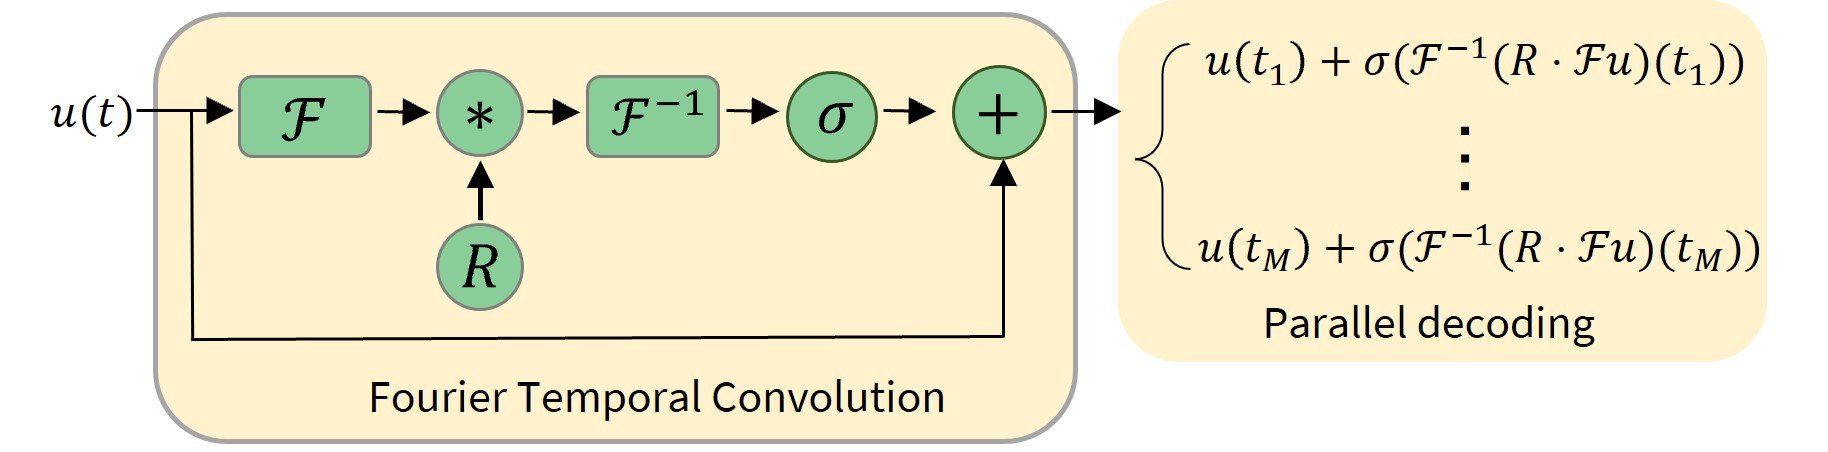
\includegraphics[width=0.98\columnwidth]{figs/parallel_decode.jpg}
%         \caption{Illustration of parallel decoding of the Fourier temporal convolution layer. Given input function $u(t)$, the Fourier coefficients $R\cdot \gF u$ are the same for all $t_i, i=1,\dots, M$. Therefore the temporal convolution layer can output the representations at different times in a single forward pass by evaluating the output function at queried points in parallel. }
%         \label{fig:parallel_decode}
% \end{figure}